\documentclass[../main.tex]{subfiles}

\begin{document}
\section{Results}
\subsection{Classification}
\subsubsection{Logistic regression on the cancer data set}
The classification problem with the breast cancer data set was done by sorting the patients into two piles. One with a cancerous tumour and one without a cancerous tumour. As said in section \ref{sec:3logreg} the data is sent into the SGD algorithm. Along with the data, there is two other variables sent into the function, amount of epochs and number of mini batches. Both the two variables have an important role on the accuracy. Therefore the accuracy was plotted as functions of the two variables, showing optimum parameters without increasing the computational complexity too much. The results from the accuracy plots can be seen in figure \ref{fig:accvsepochvsmb}. This was calculated with step sizes of 10 for both epochs and mini batches in the intervals [1-150] and [1-200].





\begin{figure}[H] 
   \centering
   \begin{subfigure}[b]{0.80\textwidth}
      \centering
    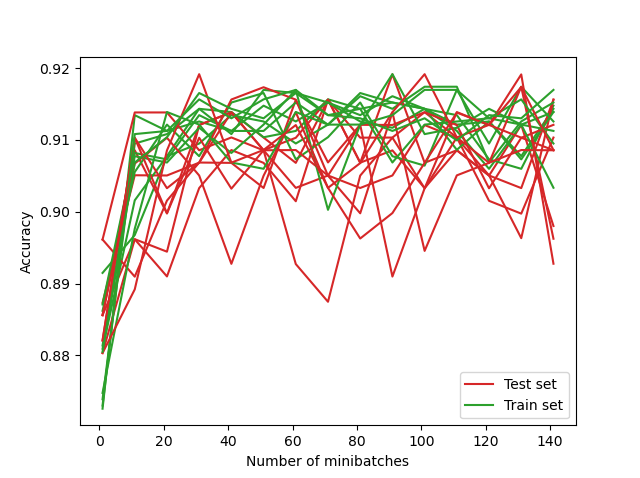
\includegraphics[width=\textwidth]{../assets/acc_vs_mb_set_40.png}
    \caption{}
    \label{fig:accvsepoch}
   \end{subfigure}
   \quad
   \begin{subfigure}[b]{0.80\textwidth}
    \centering
    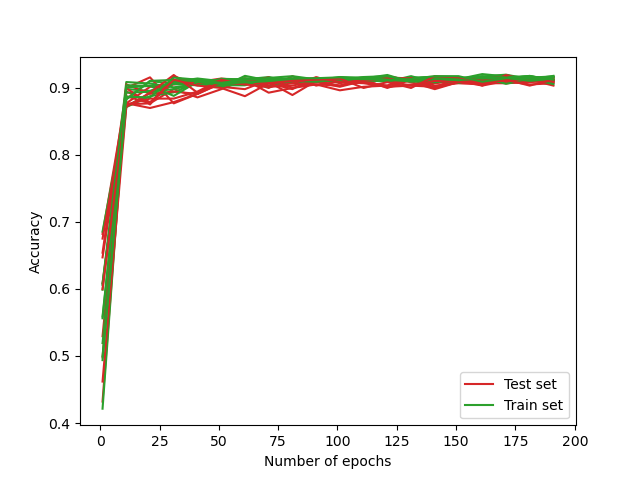
\includegraphics[width=\textwidth]{../assets/acc_vs_epoch_set_110.png} 
    \caption{}
    \label{fig:accvsmini}
   \end{subfigure}
   \caption{In both figures the calculations have been done ten times to secure a clear overview of the trend, due to some random variables as a result of the stochastic approach. (a) Plot of the accuracy vs. the number of epochs in logistic regression with constant epoch=110 (b) Plot of the accuracy vs. the number of mini batches in logistic regression with constant mini batch=40
   }
   \label{fig:accvsepochvsmb}
\end{figure} 

Regarding the classification of the data set, the chosen number of mini batches, and amount of epochs was set to 35 and 140 respectively. This was because the accuracy stops to increase around these values in figure \ref{fig:accvsepochvsmb}, without being too computational complex. 

The accuracy of the self written code applied to the Wisconsin breast cancer data set with 35 mini batches and 140 epochs gave an accuracy of 0.965. The same data set classified by scikit-learn gave an accuracy of 0.982.

Testing different amount of epochs was also done and timed to see how the increase of epochs afects the time to run the algorithms. The result of this can be seen in table \ref{tab:timetime}.


\begin{table}[H]
\centering
\caption{The time and accuracy to run the logistic regression methods with different amounts of epochs. The amount of mini batches is set to 35. The time is started when the function is called, and ends when the function is done.}
\begin{tabular}{ ccccc } 
 \toprule
  & Epochs= 140 & Epochs= 750 & Epochs= 15000 & Scikit-learn \\ 
 \midrule
 Accuracy \%  & 96.5 & 98.2 & 97.7 & 98.2\\
 
 Time (s) & 0.1562 & 0.8736 & 16.57 & 0.0030 \\ 
 \bottomrule
\end{tabular}
\label{tab:timetime}
\end{table}


\subsubsection{Neural network for classification}

\subsection{Regression}
\subsubsection{Neural network for regression}
The franke function was used as regression goal.. continue on this after lunch.

Insert the actual frankeplot here, and make sure the result pictures are correct.


\begin{figure}[htb!]
    \centering
    \begin{subfigure}[b]{0.48\textwidth}
        \centering
        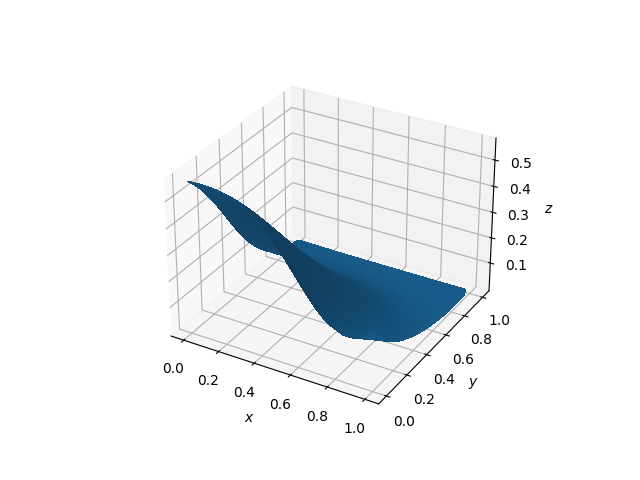
\includegraphics[trim=2.4cm 1cm 1.4cm 1cm, clip,width=1.1\textwidth]{../assets/nn_sigmoid_franke_plot.png}
        \caption{Sigmoid}
        \label{fig:result_ols_plot}
    \end{subfigure}
    \quad
    \begin{subfigure}[b]{0.48\textwidth}
        \centering
        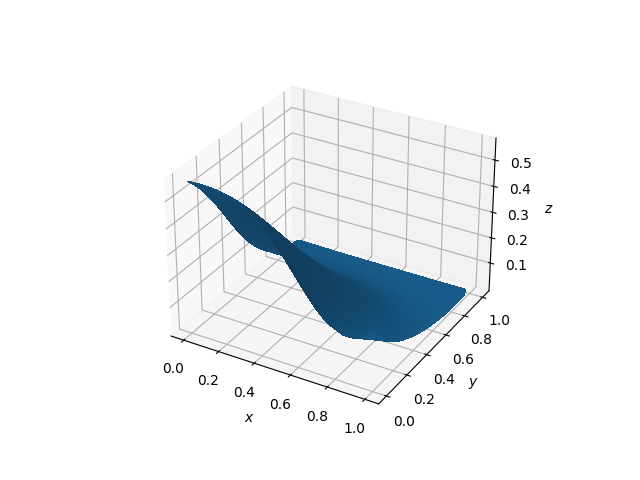
\includegraphics[trim=2.4cm 1cm 1.4cm 1cm, clip,width=1.1\textwidth]{../assets/nn_sigmoid_franke_plot.png}
        \caption{RELU}
    \end{subfigure}
    
    \begin{subfigure}[b]{0.48\textwidth}
        \centering
        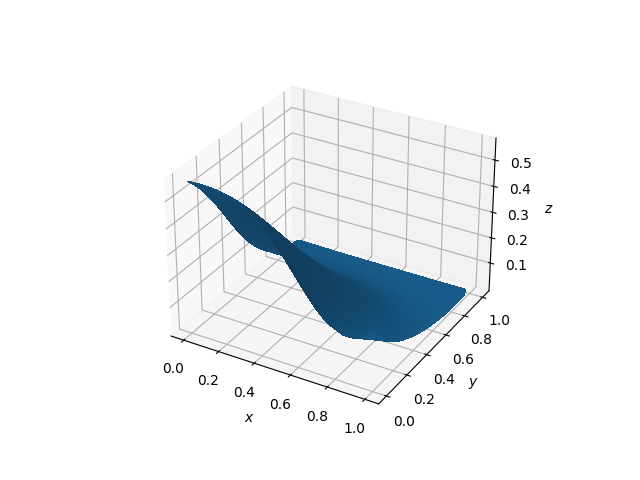
\includegraphics[trim=2.4cm 1cm 1.4cm 1cm, clip,width=1.1\textwidth]{../assets/nn_sigmoid_franke_plot.png}
        \caption{Leaky franke}
    \end{subfigure}
    \caption{Prediction of the data shown in figure \ref{fig:result_actual_plot} implementing different activation functions in the neural network}
    \label{fig:result_franke_plots}
\end{figure}



\end{document}